\documentclass{article}

\usepackage[swedish]{babel}
\usepackage{csquotes}
\usepackage[utf8]{inputenc}
\usepackage[backend=biber,style=numeric]{biblatex}
\usepackage{graphicx}
\addbibresource{kallor.bib}

\author{Michael Johansson}
\title{Harold Feinstein}

\begin{document}
\maketitle

\begin{figure}
  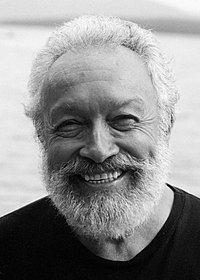
\includegraphics[width=\linewidth]{feinstein.jpg}
  \caption{Harold Feinstein}
\end{figure}

\begin{figure}
	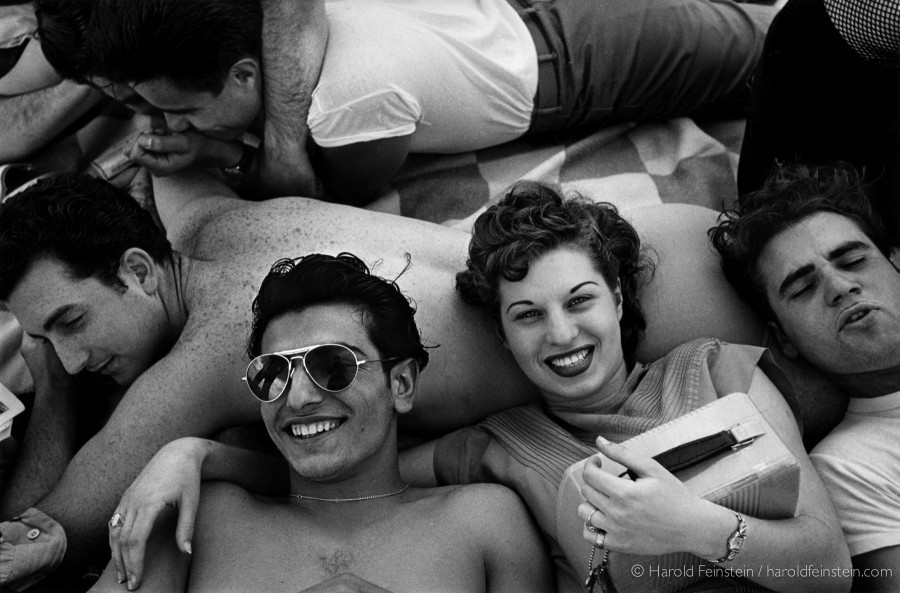
\includegraphics[width=\linewidth]{kandbild.jpg}
	\caption{En av hans mest kända bilder}
\end{figure}

\newpage

\section{Uppväxt}
Harold Feinstein föddes 1931 på Coney Island (\textcite{harsite18}) och dog den 20 Juni 2015 (\textcite{harwiki18}).
Feinsteins föräldrar var judiska invandrare, hans mamma var från Österrike och hans pappa från Ryssland (\textcite{harwiki18}).
Feinsteins första kamera hade han lånat av sin granne vid 15 års ålder.
Redan då började han sin karriär som fotograf (\textcite{harsite18}).
Efter bara fyra års fotograferande köpte den tidiga supportern Edward Steichen hans fotografier till MoMAs (Museum of Modern Arts) permanenta kollektion. (\textcite{harsite18}) detta visar på Feinsteins talang för fotografi.
Han har till och med blivit kallad \textquote{One of the most accomplished recorders of the American experience.} av \textcite{newtime15}.

\section{Karriär}
Strax efter hans första utställning på MoMA började han arbeta med W. Euguine Smith som sade detta om honom: 
\begin{displayquote}
	He is one of the very few photographers I have known or have been influenced by with the ability to reveal the familiar to me as beautifully new, in a strong and honest way.
\end{displayquote}

(\textcite{artandphoto})

En sak som jag tycker gjorde honom lite speciell var att han nästan bara använde sig av svartvita kameror, ända in i mitten på 80-talet. (\textcite{harsite18})

Hans färgfotografi var inspirerad av Louis Kahn och Frank Lloyd Wright som frågade Feinstein att fotografera deras arbete.
Feinstein har dessutom skrivit en hel del böcker, några av dessa är: \textquote{One Hundred Flowers}, \textquote{One Hundred Butterflies} och \textquote{One Hundred Seashells} om vi ska nämna några. (\textcite{harsite18})
En anledning varför jag bara nämnde hans \textquote{One Hundred}-böcker är för att han använde en speciell teknik för att få de fantastiska färgerna, det vill säga \textquote{Scanography}. (\textcite{artandphoto})
Scanography är en teknik där man använder en dokumentscanner för att ta bilderna. (\textcite{scanwiki})

Han är också väldigt känd för hans svartvita gatufotografi och hans 60år långa karriär som lärare. (\textcite{harsite18}) 

\subsection{Läraren Feinstein}
Han började som lärare redan i 20-årsåldern i New York och har lärt ut på många skolor under sin tid. Skolor som han har undervisat
på är: University of Pennsylvania’s Annenberg School of Communications, Philadelphia Museum School, School of Visual Arts, the University of Massachusetts, Maryland Institute of Art, Windham College och College of the Holy Cross. 
Han har även varit privatlärare. (\textcite{harsite18})
\newpage

\section{Bildanalys}

\begin{figure}
  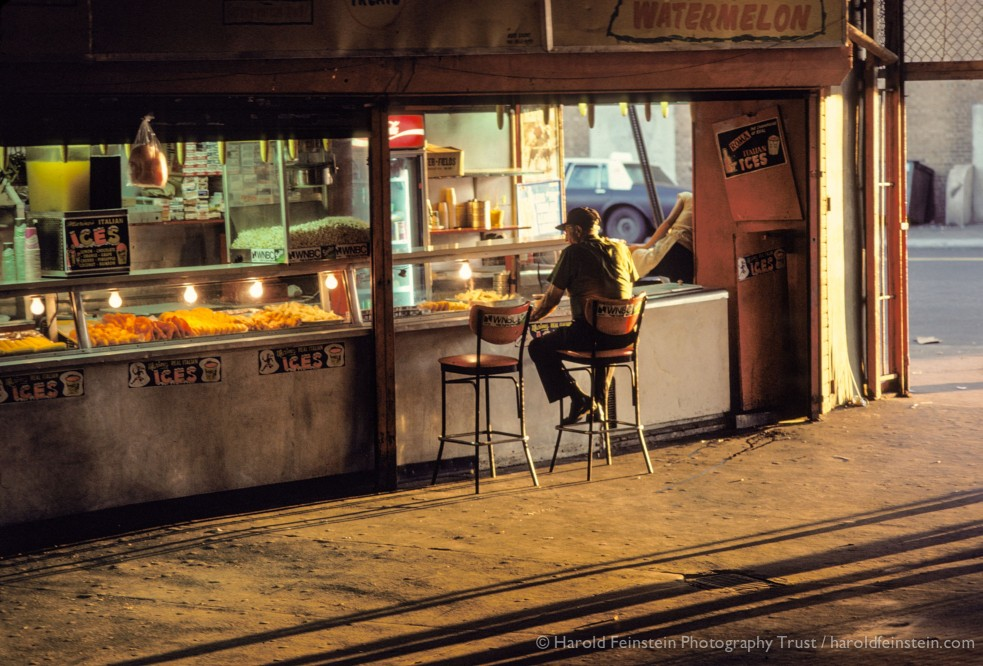
\includegraphics[width=\linewidth]{bildforanalys.jpg}
  \caption{CCI-014 Lunch Counter, 1980}
\end{figure}


Bilden heter \textquote{Lunch Counter}, den togs 1980 av Feinstein. (\textcite{harsite18})

Då detta är ett fotografi kan man säga att den representerar nutid och verklighet.
Stilen som Feinstein fotograferar i kallas \textquote{Street photography,} det är en stil där fotografen fångar ögonblicket utan att subjekten vet om det.
Man kan se att det inte är helt perfekt, personerna poserar inte riktigt på ett logiskt sätt, det är en annan sak som stödjer att bilden inte är arrangerad.
Det som kan ha varit arrangerat är tidpunkten, det ser ut som att bilden är tagen i \textquote{The golden hour}, vilket är en timme innan solen har gått ner
då ljuset är som bäst för fotografier.

Å ena sidan kan bilden vara tagen mitt på ljusa dagen med tanke på det kalla ljuset i bakgrunden till höger, å andra sidan 
kan det vara lite på kvällen, med tanke på det lite varmare ljuset från en eventuell solnedgång. Det faktum att skuggorna är långa stödjer
också teorin att det är kväll eller lite senare på dagen. Det ser ut att vara vardag då det finns en person som jobbar i gatuköket och kollar ut.
Taxin i bakgrunden ser också ut att röra på sig. Subjektet är personen som man först ser, med andra ord är det den gamla mannen som sitter framför köket. När man kollar lite närmare kan man se en till person,
denna person verkar ropa på någon som går förbi medan den gamla mannen sitter och vänter på sin mat.

Jag känner mig väldigt lugn när jag ser bilden. Ljuset i fotografiet är helt perfekt och färgerna är vackra.
Det faktum att bilden inte är arrangerad gör det hela mycket starkare, han har verkligen fångat känslorna i scenen och förmedlat dem på ett bra sätt.

Han använder sig av flera kompositionsregler:
\begin{itemize}
	\item [\bfseries{tredjedelsregeln}] En regel där man delar upp bilden i tredjedelar, både horisontellt och vertikalt
	\item [\bfseries{inramning}] En regel där man ramar en viss del av bilden för att föra fokus dit. I denna bild är tekniken mest synlig nära huvudsubjektet (den gamla mannen).
\end{itemize}

\subsection{Potentiell bakgrundshistoria}
Den gamle mannens fru dog förra året, han har fortfarande en enorm sorg efter henne och på hennes dödsdag går han alltid till hennes favoritgatukök och beställer mat åt sig själv och henne.

\section{Egna reflektioner}
Jag älskar Feinsteins bilder; kompositionen är jättebra och han lyckas verkligen förmedla en 
historia med sina bilder. Jag tycker det är kul att han använde svartvita kameror då det är
lite annorlunda. Han verkar ha haft ett intressant liv som både lärare och fotograf eftersom att han har
varit med och fotograferat allt från nöjesparker i USA och kriget i Korea.

\newpage
\printbibliography{}
\end{document}
